\section{Experiments}
\label{sec:experiments}

We run our active classifier on the above policies, and compare against machine-only and human-only baselines, as well as a baseline policy that uses a threshold-version of uncertainty sampling without any effort to minimize loss.
We report results on several datasets: CoNLL NER (restricted to PER, LOC, and O tags), Stanford sentiment classification, and a facial identification task.

While we do report runs with live humans as anecdotal evidence that the system works, using humans during comparisons introduces a set of unnecessary confounding variables. To remove ambiguity from our comparisons, and improve replicability, we also report results where we ``freeze'' the crowd by asking for a batch of labels offline, and evaluate by drawing from the human opinions (with accompanying observed delay) when the algorithm wants a human observation.
This controls for worker quality, by ensuring that all the compared approaches receive the same set of results when querying for the same human labels\footnote{If accepted, we will make our datasets of frozen human responses, delays, and worker identifier tags publicly available}.

\subsection{Three-class CoNLL Named Entity Recognition}

The CoNLL NER task asks an algorithm to distinguish between 5 possible named entity type tags for every token: \{\textbf{PER}, \textbf{LOC}, \textbf{ORG}, \textbf{MISC}, \textbf{O}\}.
We found in experiments that Turkers (and ourselves) had trouble with \textbf{MISC}, and often confused \textbf{ORG} and \textbf{LOC}, even in the presence of a detailed tutorial.

In order to minimize this confusion, we use a restricted dataset, of only \{\textbf{PER}, \textbf{LOC}, \textbf{O}\}.
Our CoNLL NER dataset is composed of 1040 sentences, drawn from the CoNLL NER training set \footnote{If accepted, we will make this dataset publicly available}.

The classifier is given 40 examples `gratis.' It is then run on the remaining 1000 sentences, drawing samples from the frozen pool of crowd responses when required, and performance is reported.

We report a set of results on a ``frozen'' dataset of crowd responses on 1000 sentences.

\begin{center}
\begin{tabular}{ | l | r | r | r | r | r | }
    \hline
    \textbf{System} & \textbf{Time/token} & \textbf{Requests/token} & \textbf{Precision} & \textbf{Recall} & \textbf{F1} \\ \hline
    Human 1-query baseline & 664 ms & 1.0 & 66.38 & 89.58 & 76.15 \\ \hline
    Human 3-query baseline & 1495 ms & 3.0 & 92.79 & 89.56 & 91.58 \\ \hline
    Human 5-query baseline & 3887 ms & 5.0 & 98.25 & 92.33 & 95.20 \\ \hline
    Offline baseline & n/a & n/a & 62.38 & 69.76 & 65.86 \\ \hline
    Threshold baseline & 1523 ms & 0.65 & 91.74 & 90.90 & 91.33 \\ \hline
    \textbf{MCTS} & 3368 ms & \textbf{0.62} & \textbf{94.32} & \textbf{93.16} & \textbf{93.73} \\ \hline
\end{tabular}
\end{center}

Anecdotally, we also report a range of results on 5 complete runs of our system using {\em real live crowd workers}, recruited at test time, over the first 150 sentences of our dataset. The results exhibit high variance based on worker quality.

\begin{center}
\begin{tabular}{ | r | r | r | r | r | }
    \hline
    Time/token & Requests/token & Precision & Recall & F1 \\ \hline
    1444 ms - 3426 ms & 0.54 - 0.66 & 92.9 - 96.91 & 82.50 - 94.01 & 87.4 - 95.43 \\ \hline
\end{tabular}
\end{center}

Filtering workers while running, or inferring separate error models for each worker, would clearly deliver substantial gains in reliability over a system that assumes uniform quality. We leave this to future work.

\subsubsection{Analysis}

To validate that this algorithm is in fact performing as we expect, we plot several graphs over the course of our run.
The red lines are true values, green is a 50 iteration floating average, and blue is a 100 iteration average.

The first thing to verify is that our system is producing consistently high accuracy, despite having a very small number of
training examples. This plot shows the F1 of the classifier, on all sentences seen so far, plotted at every sentence.
The x-axis is number of sentences seen, and the y-axis is F1 on those sentences.

\begin{figure}[t]
  \begin{centering}
  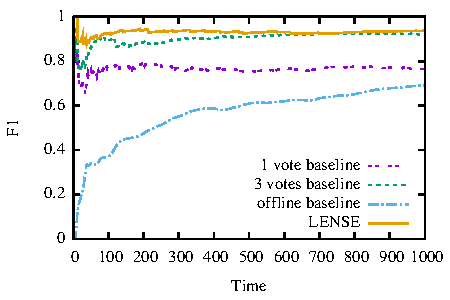
\includegraphics[width=1.0\textwidth]{figures/ner_2_class/f1_plot/f1_vs_time.pdf}
  \end{centering}
  \caption{A figure showing the comparative F1 vs time of several real-time regimes. The purple line is our system, costing just 0.65 queries per token. The green line is the 3-vote human baseline, costing 3 queries per token. The red line is the 1-vote baseline. The blue line is the performance of our classifier on its own, if we didn't allow it to query humans, and only gave it gold labels after classification in order to train.}
\label{fig:crf}
\end{figure}

The key takeaway is that our customers are receiving uninterupted, high quality service, and are completely unaware that throughout the experiment our classifier has too little data to generalize well by itself.

The second thing to verify is that we are training a good classifier over time. We held out a dev set of 300 sentences from
the CoNLL NER data that we didn't test on (ie in addition to the 1000 sentences we ran the system on). Every time we retrained
our classifier, we ran it on the this held out dev set, and plot F1. This is to demonstrate that, as expected, we can see
significant improvements in the classifier performance as soon as 1000 sentences in.

\begin{figure}[t]
  \begin{centering}
  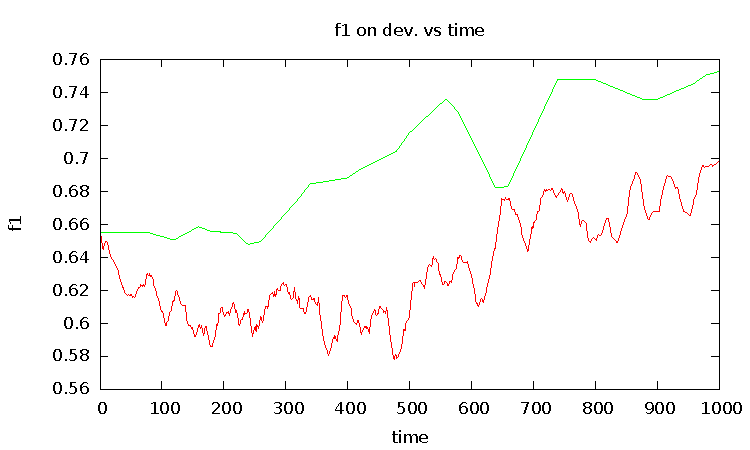
\includegraphics[width=1.0\textwidth]{figures/ner_2_class/machine_f1_plot/machine_f1_vs_time.pdf}
  \end{centering}
  \caption{A figure showing the relationship between the classifier we train, and one trained on gold labeled data. Evaluation is on a held out dev set. Note that our classifier learns more slowly because we are handing it a noisy approximation to train on, but the classifier narrows the gap as it gets more data.}
\label{fig:crf}
\end{figure}

Here the key takeaway is that even though the data we're training this classifier on introduces some noise (we never see
ground truth, just our guesses based on human observations), we are still improving our model from 65 to 70 f1 over the course
of only 1000 examples.

The third thing to verify is that our querying behavior is sound.
We don't want to see uniform querying, because that means the system isn't taking advantage of the information in our learned prior.
We also want to see a slight decrease over time, consistent with maintaining high accuracy rates.
This graph plots our queries per sentence on each iteration, normalized by sentence length.

\begin{figure}[t]
  \begin{centering}
  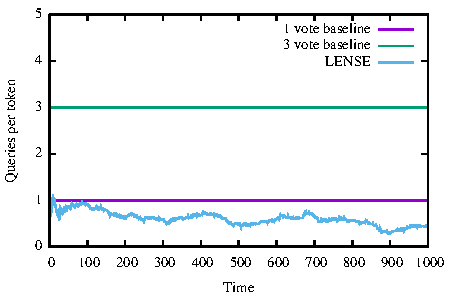
\includegraphics[width=1.0\textwidth]{figures/ner_2_class/cost_plot/cost_vs_time.pdf}
  \end{centering}
  \caption{A figure showing the number of queries required by our system, the 1 and 3 human query baselines over time.}
\label{fig:crf}
\end{figure}

This plot shows two things. First, there is high variance between sentences on how many queries are needed.
Many sentences come in with such a strong prior that they can be immediately classified, with no need to ask humans.
When querying does take place, it is generally directed towards uncertain tokens.

As a representative example of this querying behavior from the set, take observed behavior when tagging the sentence:

\begin{center}
\textit{``U.S.\ says still committed to Cuba migration pacts.''}
\end{center}

The system, having never seen the token before, starts with a belief that Cuba is 59\% Person, 37\% Location, and 3\% None. The system knows already, from previously learned examples, that ``U.S.'' is a Location with 97\% probability. It immediately fires off two queries about ``Cuba,'' and waits 4 seconds for both responses to return Location. It now believes that ``Cuba'' is a Location with 95\% probability, and decides to turn in its current guess. This guess is added to the training set, and the model is updated.

\subsection{Movie-review Sentiment Evaluation}

The Stanford Sentiment dataset \todo{Cite Jurafsky paper} consists of 2000 highly-polar movie reviews. We select a subset of 1800 of these examples to evaluate our system on, and hold out a set of 180 to evaluate intermediate classifier performance.

We start the classifier with 20 examples. We then run the classifier over 1800 examples, and report results.

We report results under two different sets of features: \{unigrams, bigrams\}, and \{unigrams, bigrams, Socher et al recursive sentence embeddings\todo{cite}\}. The comparison is designed to highlight that given a more powerful feature representation, our system is able to achieve higher accuracies for lower cost. Better modelling is not required to get high performance, as a higher spending rate can achieve that, but it does improve the achievable points on the cost-precision tradeoff curve.

\begin{center}
\begin{tabular}{ | l | r | r | r | r | }
    \hline
    \textbf{System} & \textbf{Time/example} & \textbf{Requests/example} & \textbf{Accuracy} \\ \hline
    Human 1-query baseline & 1791 ms & 1.0 & 90.79 \\ \hline
    Human 3-query baseline & 2478 ms & 3.0 & 92.20 \\ \hline
    Offline baseline - Bigrams & n/a & n/a & 70.03 \\ \hline
    Threshold baseline - Bigrams & TODO & TODO & TODO \\ \hline
    \textbf{MCTS - Bigrams} & 2853 ms & \textbf{1.83} & \textbf{93.8} \\ \hline
    Offline baseline - RNN & n/a & n/a & 85.03 \\ \hline
    Threshold baseline - RNN & TODO & TODO & TODO \\ \hline
    \textbf{MCTS - RNN} & 1926 ms & \textbf{1.48} & \textbf{93.1} \\ \hline
\end{tabular}
\end{center}

\subsubsection{Analysis}

This is a graph of the relative cost per example over time, for the basic features (green) and the rich RNN embedding features (red):

\begin{figure}[t]
  \begin{centering}
  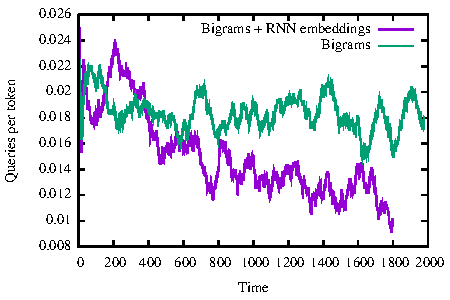
\includegraphics[width=1.0\textwidth]{figures/sentiment_cost_per_token_vs_time/cost_per_token_vs_time.pdf}
  \end{centering}
  \caption{A figure showing that increasing model capacity with richer distributional features (red line) enables the model to reduce costs further over time, compared with a simpler bag-of-words model with less representational capacity (green line).}
\label{fig:crf}
\end{figure}

The thing to note is that although accuraccy rates remain high for both approaches throughout, the richer model is able to learn more over time, and subsequently costs the operator of our system less.

\subsection{Facial Identification Evaluation}

The Facial Identification task we investigate uses a constructed subset of a dataset of online photos of celebrities\todo{Princeton something-or-other}. The task we evaluate on is a 4-way facial recognition task, choosing from one of four celebrities \{Anderson Cooper, Daniel Craig, Scarlet Johansson, Miley Cyrus\}, starting with 1 training example per person. We use the last layer of an 11-layer AlexNet trained on ImageNet as input embeddings to featurize each of the images.

\begin{center}
\begin{tabular}{ | l | r | r | r | r | r | }
    \hline
    \textbf{System} & \textbf{Time/example} & \textbf{Requests/example} & \textbf{Accuracy} \\ \hline
    Human 1-query baseline & 1414 ms & 1.0 & 87.75 \\ \hline
    Human 3-query baseline & 1865 ms & 3.0 & 88.44 \\ \hline
    Offline baseline & n/a & n/a & 87.43 \\ \hline
    Threshold baseline & TODO & TODO & TODO \\ \hline
    \textbf{MCTS} & 2042 ms & 1.06 & 88.45 \\ \hline
\end{tabular}
\end{center}

\todo{write}

